\documentclass[12pt, letterpaper]{article}

\usepackage[margin=1.25in]{geometry}
\usepackage{amsmath, amssymb}
\usepackage{graphicx}
\usepackage{authblk}
\usepackage{indentfirst}
\usepackage{blindtext}
\usepackage{hyperref}
\graphicspath{{./Images/}}
\setlength{\parindent}{12pt}
\setlength{\parskip}{1em}

\title{STAT131 Ch.1 Notes}
\author{William Santosa}
\date{Winter 2022 Quarter}

\begin{document}

\maketitle

\section{Introduction}
This document covers essential information and example problems with answers in Chapter 1 in the "Introduction to Probability, 2nd Edition" written by Joseph K. Blitzstein and Jessica Hwang.

\section{Important Definitions}

Contains important definitions for understanding Chapter 1 in textbook.

\begin{itemize}
    \item \textit{Sample Space S} is the set of all possible outcomes from the experiment.
    \item \textit{Event A} is the subset of \emph{sample space} S.
    \begin{itemize}
        \item \textbf{Note:} We say an event \textit{occurred} if the actual outcome is in A.
    \end{itemize}
    \item \textit{Complement} of A are the elements not in A, denoted as \[A^{c}\]
    \item \textit{Union} of A and B occurs if \textit{at least one} of A or B occurs \[A \cup B\]
    \item \textit{Intersect} of A and B occurs if only and if \textit{both} of A and B occur \[A \cap B\]
    \item \textit{De Morgan's laws} are a pair of transformation rules vital to set theory \[(A\cup B)^{c} = A^{c}\cap B^{c}\text{ and } (A\cap B)^{c} = A^{c}\cup B^{c}\]
    \item \textit{Naive definition of probability} is to count the number of ways an event can happen and divide by the total number of possible outcomes \[P_{naive}(A) = \frac{|A|}{|S|} = \frac{\text{number of outcomes favorable to A}}{\text{total number of outcomes in S}} \]
    \begin{enumerate}
        \item There is \textit{symmetry} in the problem if outcomes are equally likely.
        \item Naive can be used when outcomes are equally likely \textit{by design}.
        \item Naive is useful as a \textit{null model}, which is when we apply the naive definition to see what predictions it would yield.
    \end{enumerate}
    \item The \textit{multiplication rule} is used for \textit{sampling with replacement} and \textit{sampling without replacement}.
    \begin{itemize}
        \item \textbf{Usage:} Compound experiment with experiment A, B, with a, b outcomes respectively. Then the compound experiment has \textit{ab} possible outcomes.
    \end{itemize}
    \item To adjust for overcounting, note the amount of times you count each probability (c) and adjust by dividing by c.
    \item \textit{Story proofs} are proofs by interpretation. This usually means counting the same thing in two different ways, rather than doing an algebraic proof.
    \item A \textit{probability space} consists of a sample space S and a \textit{probability function} P that takes an event A is a subset of S as input and returns \textit{P(A)}, a real number between 0 and 1, inclusive, as output. It must satisfy the following axioms.
    \begin{enumerate}
        \item \(P(\emptyset) = 0\), \(P(S) = 1\).
        \item If \(A_{1}, A_{2},\) ... are disjoint events, then \[P(\bigcup\limits_{j=1}^{\infty}(A_{j})) = \sum\limits_{j=1}^{\infty}P(A_{j}).\]
    \end{enumerate}
    \item For any events A and B, they hold the properties:
    \begin{enumerate}
        \item \(P(A^{c}) = 1 - P(A) \)
        \item If \(A \subset B \), then \(P(A) \leq P(B) \)
        \item \(P(A \cup B) = P(A) + P(B) - P(A \cap B) \)
    \end{enumerate}
    \item \textit{Permutations} occur when \underline{selecting without replacement} and \underline{order is important}
    \begin{itemize}
        \item \textbf{Usage: }\(\frac{n!}{(n - k)!} \), n = total number of items, k = number of chosen items, denoted as \(_{n}P_{k}, P(k, n), P_{n, k}\)
    \end{itemize}
    \item \textit{Combinations} occur when \underline{selecting without replacement} and \underline{order isn't important}
    \begin{itemize}
        \item \textbf{Usage: }\(\frac{n!}{(n - k)!k!} \), n = total number of items, k = number of chosen items, denoted as \(_{n}C_{k}, C(k, n), C_{n, k}  \)
    \end{itemize}
    \item Choosing an item \textit{with replacement} means you can choose the same item multiple times
    \begin{itemize}
        \item \textbf{Usage: }\(n^{k}\), n = total number of items, k = number of chosen items
    \end{itemize}
\end{itemize}

\section{Screenshots}
\begin{enumerate}
    \item 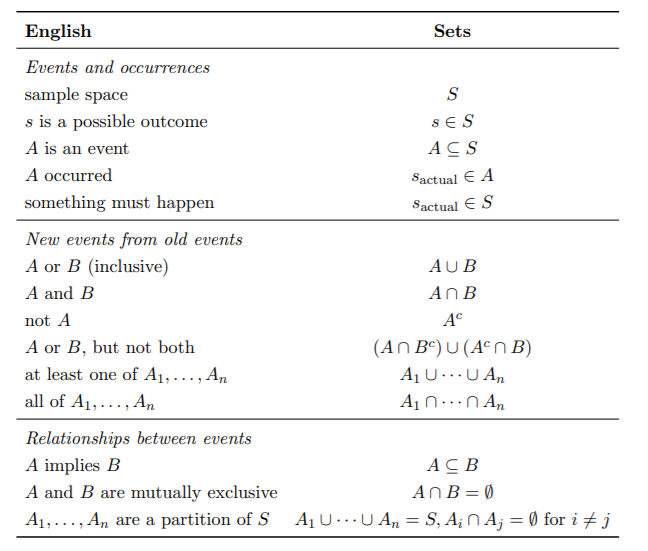
\includegraphics{English.png}
    \item 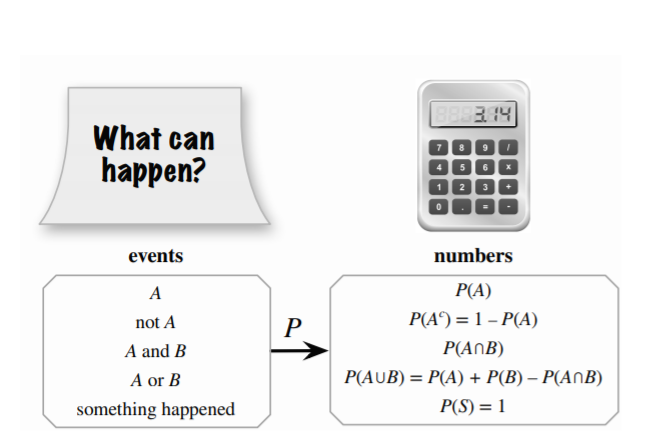
\includegraphics{Happen.png}
    \item 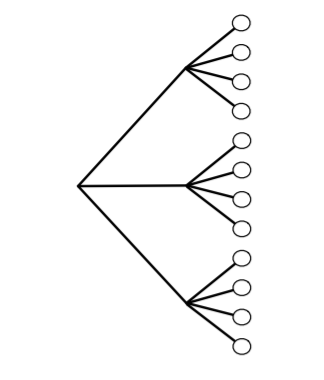
\includegraphics{Tree.png}
\end{enumerate}

\end{document}